\section{Approach}
\label{sec:approach}

To reason about causality between short texts,
our framework includes i) a network of causal relation weighted with
causality co-occurrences between terms that is extracted from
a large web corpus; ii) a novel metric to compute causal strength
 between any two terms based on this network; iii)
a simple algorithm for aggregating the causality between terms to
compute the overall score for causality reasoning between short texts,
including phrases and sentences.
Next, we describe these components.

\subsection{Causality Network}
\label{sec:network}

Causality exists in natural language sentence and can be identified by
linguistic patterns known as {\em causal cues}~\cite{ChangC04}.
Consider the following sentences:
%\small{
\enumsentence{\shortex{5}
		{ The & {\em \underline{storm}} & [{\bf caused}] & a tremendous amount of & {\em \underline{damage}} }
        { & {\sc cause} & {\sc pattern} & & {\sc effect} }
        {on the landing beaches.}
		}
%}
\enumsentence{ The team prepared GIS precipitation and contour maps of the area
identifying the
\shortex{5}{{\em \underline{flooding}} & and landslides & [{\bf caused by}]
 & the & {\em \underline{rainfall}}.}
{ {\sc effect} & & {\sc pattern} & & {\sc cause}} {}
}
\enumsentence{
\shortex{5}{However Susanoo was in & {\em \underline{sorrow} } & after the & {\em \underline{loss} } & of his}
{& {\sc effect} & & {\sc cause} &}
{ mother and he was raging in his kingdom. }
}

In sentence (1),
`storm' is the cause of `damage', and `damage' is the effect of `storm'.
We exploit {\em causal cues} (causal patterns) shown in \tabref{tab:cue},
to identify cause and effect roles for our causality knowledge.
For example, \textit{``A cause B''} is an intra-sentence causal
cue where \textit{A} is a text span that represents the cause
and \textit{B} is a span that represents the effect.
We set a maximum length $L$
of text span \textit{A} and \textit{B} to prevent
extracting noisy pairs too far away from causal cues.\footnote{In our
experiments, we empirically set $L$ to be 10.}
The text span can be a term, a phrase or a sentence.
There are also discourse cues such as \textit{``If A then B''}.
\tabref{tab:cue} shows all 53 intra-sentence and discourse
causal cues used in this work.
We extract all such patterns from a large web corpus, and after lemmatization,
pair each term $i$ in $A$ as cause role, denoting as $i_c$, with each term $j$
in $B$ as effect role, denoting as $j_e$, to form a list of
\textit{causal pairs} $(i_c,j_e)$ as causal evidences.
Therefore, from sentence (1), we can harvest
$(\text{storm}_{\text{c}}, \text{tremendous}_{\text{e}})$,
$(\text{storm}_{\text{c}}, \text{amount}_{\text{e}})$,
$(\text{storm}_{\text{c}}, \text{damage}_{\text{e}})$,
$(\text{storm}_{\text{c}}, \text{landing}_{\text{e}})$,
and $(\text{storm}_{\text{c}}, \text{beach}_{\text{e}})$
as causal evidences.
In this process, we remove the stop words and only pairs involving nouns, verbs,
adjectives and adverbs from WordNet are retained.

Our extracted causal pairs form a {\em directed} network of causal relations.
Each node in this network is a lemmatized term,
while a directed edge between two terms indicates a causal relation.
A fragment of the causal network with three words in the network is
shown in \figref{fig:causalnet}.
Each edge is annotated with the {\em causality co-occurrences}, i.e.,
the number of times this causal relation was observed in the corpus.

\begin{table*}[th]
\centering
\caption{53 Causal cues. \textit{A} is a cause span, and \textit{B} is an effect span.
DET stands for a/an/the/one. BE stands for is/are/was/were.}
\label{tab:cue}
\resizebox {\textwidth}{!}{
\begin{tabular}{|l l l|l l l|}
\hline \multicolumn{3}{|c|}{intra-sentence} & \multicolumn{3}{c|}{inter-sentence}\\
\hline \hline

A lead to B & A leads to B & A led to B & If A, then B& If A, B & B, because A \\
A leading to B & A give rise to B & A gave rise to B & B because A & B because of A & Because A, B \\
A given rise to B & A giving rise to B & A induce B & A, thus B & A, therefore B & B, A as a consequence \\
A inducing B & A induces B & A induced B & Inasmuch as A, B & B, inasmuch as A & In consequence of A, B \\
A cause B & A causing B & A causes B & B due to A & Due to A, B & B in consequence of A \\
A caused B & B caused by A & A bring on B & B owing to A & B as a result of A & As a consequence of A, B\\
A brought on B & A bringing on B & A brings on B & A and hence B & Owing to A, B& B as a consequence of A\\
B result from A & B resulting from A &  B results from A & A, hence B & A, consequently B & A and consequently B\\
B resulted from A & \multicolumn{2}{l|}{the reason(s) for/of B BE A} & \multicolumn{3}{l|}{A, for this reason alone , B} \\
DET effect of A BE B &\multicolumn{2}{l|}{A BE DET reason(s) of/for B} & & & \\
\hline
\end{tabular}}
\end{table*}

We choose to extract term pairs in a rather simplistic way, without deeper
syntactic analysis, because i) we opt for breadth in the causal knowledge
hence the input corpus is extremely large (around 10TB), and consequently
deep parsing of the text becomes prohibitive; and ii) the sheer quantity of
the term pairs thus obtained provides excellent statistics for us to
distinguish true causal relations against false ones.

\begin{figure}[th]
\centering
%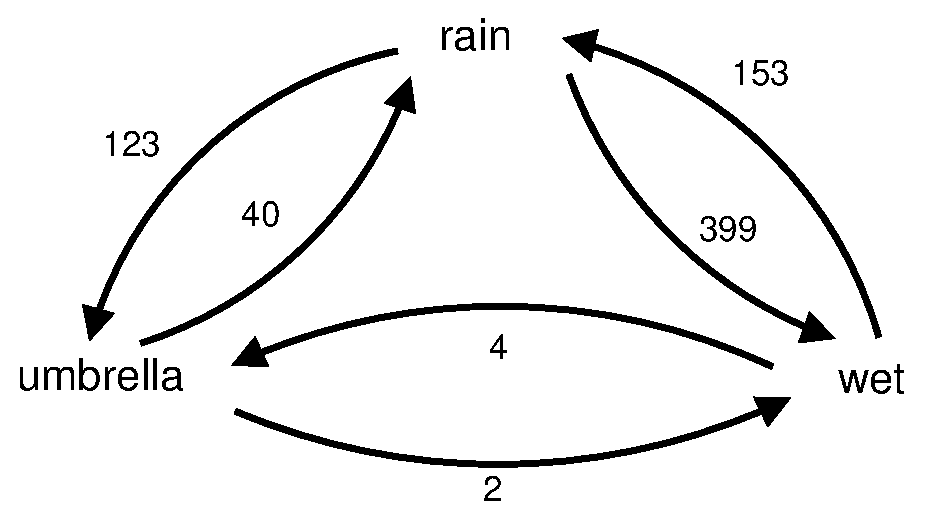
\epsfig{file=causalnet.eps, width=0.6\columnwidth}
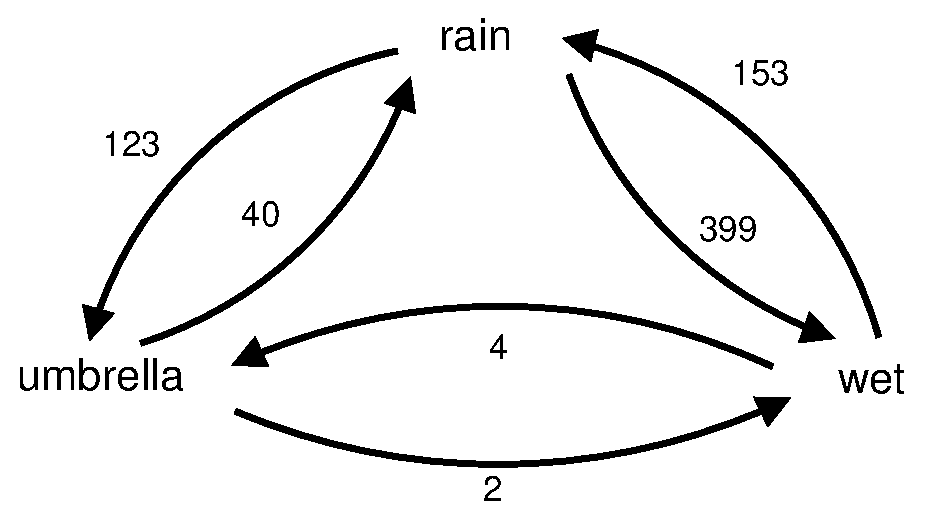
\includegraphics[width=0.7\columnwidth]{causalnet}
\caption{A fragment of causal network}
\label{fig:causalnet}
\end{figure}

\subsection{Causal Strength Computation}
\label{sec:causalstrength}

Text corpus can explicitly as well as implicitly encode causality.
Explicit causality is represented in text
with causal patterns or indicators (e.g., cause, because).
Implicit causality is naturally encoded in discourse without indicators, e.g.,
$A$ appears before $B$ in discourse implies that $A$ is a cause of $B$,
which is more complex and difficult to recognize.
For example,
sentence (1) and (2) explicitly encode causalities using causal patterns,
while sentence (3) encodes the implicit causality
$(\text{loss}_{\text{c}}, \text{sorrow}_{\text{e}})$.

Gordon et al.~\shortcite{gordon2011commonsense} collected implicit causality
from personal story corpus using asymmetric PMI described by Church\shortcite{church1990word},
to achieve the previous best known result on COPA task.
The intuition is that narrations typically describe a series of events
ordered by time. The text that appears earlier may be the antecedent
while the text that comes later may be the consequent.
Therefore, asymmetric PMI statistics can be used to capture
the implicit causalities encoded in narrative texts such as personal stories.
However, while personal stories might be a good source of implicit causality,
they are hard to come by and limited in scale.
In contrast, using a larger general web corpus improves coverage but
trading accuracy, as web sentences may not follow a narrative pattern.

To leverage the scale and richness of the web text,
we model causality more properly by replacing lexical co-occurrences with
causality co-occurrences extracted by causal cues.
Lexical co-occurrences are weak and implicit causal evidences,
while causality co-occurrences are stronger and more explicit causal
evidences due to the use of causal cues.
Causal cues also help to identify precise cause/effect roles in
strong causal evidences.
Then we propose a new metric to measure causal strength between
two terms with the insight that the connotation of causality
integrates \emph{necessity causality}
with \emph{sufficiency causality}.
Considering a causal pair $(i_c,j_e)$,
necessity causality encoded by $(i_c, j_e)$ represents
that the cause $i$ {\em must} be present in order for
the effect $j$ to take place,
while sufficiency causality encoded by $(i_c, j_e)$ represents
that cause $i$ is all it takes bring about the effect $j$.
For example, the causality $(\text{rainfall}_{\text{c}}, \text{flooding}_{\text{e}})$
in sentence $(2)$  encodes more necessity causality,
since the effect \textit{flooding} cannot happen
if \textit{rainfall} did not happen as its cause.
Similarly, $(\text{storm}_{\text{c}}, \text{damage}_{\text{e}})$ in
sentence $(1)$ encodes more sufficiency causality.
Intuitively, the stronger the necessity causality is, the larger
the $p(i_c|j_e)$ should be;
the stronger the sufficiency causality is, the larger
the $p(j_e|i_c)$ should be.
We are able to compute such conditional probability because we distinguish
the terms by cause or effect roles. However, the popular terms are
more likely to be extracted as either causes or effects,
which makes the conditional probability metric bias toward
highly frequent terms.
Therefore, we adopt a more general form (with a penalty factor)
to model the necessity causal strength and
sufficiency causal strength encoded by $(i_c,j_e)$,
as shown in \eqnref{eq:csnec} and \eqnref{eq:cssuf} respectively.

\begin{align}
CS_{nec}(i_c,j_e)  & =  \frac{p(i_c|j_e)}{p^{\alpha}(i_c)} \nonumber \\
                   & = \frac{p(i_c,j_e)}{p^{\alpha}(i_c)p(j_e)}
\label{eq:csnec}
\end{align}
\begin{align}
CS_{suf}(i_c,j_e) & = \frac{p(j_e|i_c)}{p^{\alpha}{j_e}} \nonumber \\
                  & = \frac{p(i_c,j_e)}{p(i_c)p^{\alpha}(j_e)}
,\label{eq:cssuf}
\end{align}
where $\alpha$ is a constant penalty exponent value.
We follow Wettler~\shortcite{Wettler:1993} to set $\alpha$ to be $0.66$,
penalizing high-frequency response terms.
$p(i_c)$, $p(j_e)$ and $p(i_c,j_e)$ are computed as follows:
\begin{equation}
p(i_c) = \frac{\sum_{w\in W}
f (i_c,w_e)}{M}
\end{equation}
\begin{equation}
p(j_e) = \frac{\sum_{w\in W}
f (w_c,j_e)}{M}
\end{equation}
\begin{equation}
p(i_c,j_e) = \frac{f(i_c,j_e)}{N}
\end{equation}
Here, $f(i_c,j_e)$ is frequency of observing the causal pair
$(i_c,j_e)$
from the corpus; $M$ is the total number of evidences, computed as:
$$\sum_{u\in W} \sum_{v\in W} f(u_c,v_e),$$
and $N$ is the size of the corpus;
$W$ is the set of all terms in the causality network.

To show the effectiveness of $CS_{nec}$ and $CS_{suf}$,
we compute the necessity causality and suffiency causality
for causal pairs annotated in SemEval-2010 task 8.\footnote{We further
discuss this corpus in \secref{sec:eval}}
We show the top necessary causal pairs and sufficient causal
pairs ranked by $\frac{CS_{nec}}{CS_{suf}}$ and $\frac{CS_{suf}}{CS_{nec}}$
respectively as shown in \tabref{tab:necsuf}.
% insert the fig:necsuf here
\begin{table}[th]
\caption{Top necessary and sufficient causal pairs}
\label{tab:necsuf}
%\small
\begin{tabular}{l|l}
%\hline intra-sentence cue & inter-sentence cue  \\
Necessary Causal Pairs & Sufficient Causal Pairs \\
\hline \hline
$(\text{man}_c, \text{kidnapping}_e)$ & $(\text{neuroma}_c, \text{pain}_e)$ \\
$(\text{man}_c, \text{jolliness}_e)$ & $(\text{eyestrain}_c, \text{headache}_e)$ \\
$(\text{wind}_c, \text{corkscrew}_e)$ & $(\text{flashlight}_c, \text{light}_e)$ \\
$(\text{rainfall}_c, \text{flooding}_e)$ & $(\text{typhoon}_c, \text{damage}_e)$ \\
$(\text{accident}_c, \text{snarl}_e)$ & $(\text{sunrise}_c, \text{light}_e)$ \\
$(\text{erosion}_c, \text{rill}_e)$ & $(\text{claustrophobia}_c, \text{panic}_e)$ \\
$(\text{crash}_c, \text{gash}_e)$ & $(\text{quake}_c, \text{damage}_e)$\\
$(\text{virus}_c, \text{tonsillitis}_e)$ & $(\text{bacteria}_c, \text{meningitis}_e)$  \\
$(\text{fight}_c, \text{carnage}_e)$ & $(\text{quake}_c, \text{loss}_e)$ \\
$(\text{earthquake}_c, \text{avalanche}_e)$ & $(\text{overproduction}_c, \text{growth}_e)$ \\
\hline
\end{tabular}
\end{table}

Our new causal strength encoded by pair $(i_c,j_e)$ combines
$CS_{nec}(i_c,j_e)$ with $CS_{suf}(i_c,j_e)$,
and is defined in \eqnref{eq:weightedcs}.
\begin{equation}
CS(i_c,j_e) = CS_{nec}(i_c,j_e)^{\lambda} CS_{suf}(i_c,j_e)^{1-\lambda}
%&= \left(\frac{p(i_c|j_e)}{p^{\alpha}(i_c)}\right)^{\lambda}\left(\frac{p(j_e|i_c)}{p^{\alpha}(j_e)}\right)^{1-\lambda}
\label{eq:weightedcs}
\end{equation}
The above metric models both the necessity and sufficiency components
of causality and captures the intuition that
the causal strength should be stronger when both necessity and sufficiency
causality are strong.
Here, $\lambda$ is a parameter, weighing the necessity and sufficiency
causality knowledge that is extracted from text corpus.
A desirable $\lambda$ depends on the characteristics of knowledge
source and extraction methods, as we show in Section~\ref{sec:eval}.

We compute the causal strength between every pair of terms in the
causality network
according to \eqnref{eq:weightedcs}. Where an edge is missing in the network,
we assign a causal strength of zero.

\subsection{Commonsense Causal Reasoning}
\label{sec:reasoning}

To compute whether alternative $a_1$ or $a_2$ is more plausible
with respect to the premise $p$, we need to compare the overall causality
strength $CS_T(p,~a_1)$ and $CS_T(p,~a_2)$, assuming $p$ is asking
for an effect. Here, we compute the causal strength from
text $T_1$ to text $T_2$ as:
\begin{equation}
CS_T(T_1,T_2)=\frac{1}{|T_1|+|T_2|}\sum_{i \in T_1}\sum_{j \in T_2}
CS(i, j)
\label{eq:csall}
\end{equation}

We argue that such simple approach to aggregate causal strength between terms
can effectively model causality between short texts.
The intuition is that each pair of terms drawn from the two texts contribute
to the total causal strength between the two texts. Because $CS(i_c, j_e)$
can be closely related to a probability (with penalty factors),
summing up the causal strength between all pairs is analogous to
computing a pairwise disjunctive probablity.

Furthermore, in our causality model, each term, whether in the cause role
or the effect role, acts as an active agent in contributing causal strength,
either in $CS_{nec}$ or $CS_{suf}$. Each term in the cause role may
cause a number of terms in the effect role and each term in the effect role
maybe caused by a number of terms in the cause role.
Based on this one-to-many relation, we normalize total causality score by
$|T_1|+|T_2|$, which is the total number of agents,
and not $|T_1|\times|T_2|$ presented in previous papers.

One alternative way of constructing the causality network is to extract
causal pairs between phrases instead of terms, since there exists complex
events (e.g., ``catch cold'') that cannot be expressed by a single word.
However, we empirically discovered that such network is less
effective since the frequencies tend to be diluted,
which we report in Section~\ref{sec:eval}, and even though ``catch cold''
is not in our network, we could better capture
phrase causality based on the combined contribution of individual words
``catch'' and ``cold.''
